\documentclass[12pt,a4paper]{article}

% ---- Packages ----
\usepackage[utf8]{inputenc}
\usepackage[T1]{fontenc}
\usepackage{lmodern}
\usepackage[margin=1in]{geometry}
\usepackage{amsmath,amssymb,mathtools,bm}
\usepackage{graphicx}
\usepackage{float}
\usepackage[dvipsnames]{xcolor}
\usepackage{tikz}
\usetikzlibrary{arrows.meta,calc,decorations.markings,patterns,3d}
\usepackage{pgfplots}
\pgfplotsset{compat=1.17}
\usepackage{booktabs}
\usepackage{caption}
\usepackage{setspace}
\usepackage{fancyhdr}
\usepackage{microtype}
% Paragraph formatting: skip + indent (no indent after section titles)
\setlength{\parskip}{6pt}
\setlength{\parindent}{15pt}
\makeatletter
\let\orig@section\section
\renewcommand{\section}{\@ifstar{\orig@section*}{\@dblarg{\my@section}}}
\def\my@section[#1]#2{\orig@section[#1]{#2}\noindent\@afterindentfalse\@afterheading}
\let\orig@subsection\subsection
\renewcommand{\subsection}{\@ifstar{\orig@subsection*}{\@dblarg{\my@subsection}}}
\def\my@subsection[#1]#2{\orig@subsection[#1]{#2}\noindent\@afterindentfalse\@afterheading}
\makeatother
\usepackage[numbers,sort&compress]{natbib}
\usepackage{hyperref}
\usepackage{cleveref}

\hypersetup{
  colorlinks=true,
  linkcolor=NavyBlue,
  citecolor=NavyBlue,
  urlcolor=NavyBlue
}

\setstretch{1.0}

\pagestyle{fancy}
\fancyhf{}
\rhead{\thepage}
\lhead{\textit{Toroidal Manifolds and Recursive Neural Dynamics}}
\renewcommand{\headrulewidth}{0.4pt}

% ---- Title ----
\title{\textbf{Toroidal Manifolds and Recursive Neural Dynamics:\\
A Physical Framework for Self-Referential\\Information Processing}}
\author{Christopher Ezernack\\
\textit{Department of Physics and Cognitive Science}\\
\textit{University of Texas at Dallas}\\
\texttt{christopher.ezernack@utdallas.edu}}
\date{\today}

\begin{document}
\maketitle
\thispagestyle{empty}

\begin{abstract}
Gardner et al.\ (2022) demonstrated that the joint population activity of grid cells in the medial entorhinal cortex resides on a toroidal manifold $T^2 = S^1 \times S^1$. This result provides the first direct empirical evidence that neural computation evolves on non-trivial topological attractor geometries.

This paper develops a physical framework explaining why toroidal manifolds arise in recursive neural systems. Coupled oscillatory processes naturally produce toroidal attractors in phase space, consistent with the Kolmogorov--Arnold--Moser theorem for quasi-periodic motion. The electromagnetic spectrum serves as the base physical layer, with particular attention to the measurement gap between conventional electrophysiology (Hz to kHz) and molecular vibrational dynamics ($10^{9}$ to $10^{13}$~Hz). Quaternion rotations provide a natural mathematical representation of coupled phase dynamics on higher-dimensional tori, and entropy gradients constrain neural activity onto low-dimensional attractor manifolds.

The framework connects these dynamical principles to the emergence of modular oscillatory organization, the evolutionary pressures that shaped recursive internal modeling in the nervous system, and the transition to self-referential information processing. Testable predictions are presented for each component of the framework.
\end{abstract}

\newpage

%% ============================================================
%% SECTION 1: INTRODUCTION
%% ============================================================
\section{Introduction}\label{sec:intro}

\subsection{Grid Cells and Continuous Attractor Networks}

The discovery that grid cells in the medial entorhinal cortex fire in characteristic hexagonal spatial patterns \cite{Hafting2005} established that the mammalian brain contains a structured internal coordinate system for spatial representation. This finding, which contributed to the Nobel Prize in Physiology or Medicine awarded to May-Britt Moser and Edvard I.\ Moser, revealed that individual grid cells fire at the vertices of a regular triangular lattice as an animal traverses an environment. Grid cells are organized into discrete modules, each with a characteristic spatial scale, and the ratio of scales between adjacent modules follows an approximately constant geometric factor \cite{Stensola2012}. The spatial code of a single grid cell can be described by two circular phase variables, meaning that the state space of an individual cell's firing pattern is inherently periodic.

Theoretical models proposed that grid cell networks implement continuous attractor dynamics, in which the population activity evolves on a low-dimensional manifold embedded in the high-dimensional space of possible firing rate vectors \cite{Yoon2013}. In a continuous attractor network, the set of stable states forms a connected manifold rather than a collection of isolated fixed points, and the system can move smoothly along this manifold in response to velocity inputs. For a two-dimensional periodic spatial code, the predicted attractor manifold is a two-dimensional torus $T^2 = S^1 \times S^1$.

\subsection{The Gardner et al.\ Discovery}

The decisive empirical confirmation came from Gardner et al.\ \cite{Gardner2022}, who recorded simultaneously from large populations of grid cells in individual modules of the rat medial entorhinal cortex. Using persistent cohomology, a technique from topological data analysis that can recover the topology of a manifold from a finite point cloud, they reconstructed the shape of the manifold on which the population activity resides. The analysis revealed that the joint activity of grid cells within a single module traces a path on a two-dimensional torus $T^2 = S^1 \times S^1$.

This result was significant for several reasons. It provided the first direct visualization of continuous attractor network dynamics in the brain. It confirmed that neural population activity can be organized on non-trivial topological manifolds. It demonstrated that the tools of algebraic topology can be applied to experimental neural data to recover geometric structure that is not visible in the activity of individual neurons.

\subsection{Why Toroidal Geometry Matters}

The toroidal structure observed in grid cell populations is not an isolated property of the spatial navigation system. From the perspective of dynamical systems theory, toroidal manifolds arise naturally whenever multiple oscillatory processes interact. A single periodic process traces a circle $S^1$ in phase space; two coupled periodic processes trace a torus $S^1 \times S^1$; and $n$ interacting oscillatory variables produce an $n$-dimensional torus $T^n$ \cite{Strogatz2015}. The Kolmogorov--Arnold--Moser (KAM) theorem establishes that such quasi-periodic toroidal motion persists under small perturbations of integrable Hamiltonian systems \cite{Kolmogorov1954, Arnold1963, Moser1962}, providing a rigorous mathematical foundation for the structural stability of these manifolds.

Neural systems contain the oscillatory dynamics needed to produce toroidal attractors. Electroencephalographic recordings reveal rhythmic activity spanning multiple frequency bands, from slow delta oscillations ($<4$~Hz) through theta (4--8~Hz), alpha (8--13~Hz), beta (13--30~Hz), and gamma ($>30$~Hz) rhythms \cite{Buzsaki2006, Buzsaki2004}. These oscillations interact through cross-frequency coupling mechanisms, notably theta-gamma phase-amplitude coupling observed in the hippocampus and neocortex \cite{Canolty2006, Tort2009, Lisman2005}. Such coupled oscillatory dynamics provide the conditions under which toroidal attractor manifolds are expected to emerge.

\subsection{Goal of This Paper}

This paper develops a physical dynamical framework explaining why toroidal manifolds arise in recursive neural systems. The argument proceeds through several layers: grid cell evidence as the empirical anchor, oscillatory neural dynamics, the mathematical construction of toroidal manifolds, KAM stability, and quaternion representations of multi-band phase dynamics. It continues with the terahertz measurement gap, evolutionary pressure from the gut microbiome, the Jaynesian transition, and entropy-constrained attractor dynamics. The conclusion connects these threads to recursive self-reference consistent with G"{o}del-type logical structure \cite{Godel1931, Hofstadter1979}.

The central claim is not that toroidal attractor dynamics fully explain consciousness. Rather, the paper argues that recursive oscillatory systems naturally produce toroidal attractor manifolds in phase space. Neural systems contain the coupled oscillatory dynamics necessary for such manifolds to emerge, and the grid cell system provides a concrete empirical demonstration of this principle.


%% ============================================================
%% SECTION 2: GRID CELLS AND TOROIDAL MANIFOLDS
%% ============================================================
\section{Grid Cells and Toroidal Manifolds}\label{sec:grid_cells}

\subsection{Continuous Attractor Networks and Neural Manifolds}

The theoretical framework of continuous attractor neural networks (CANNs) provides the foundation for understanding toroidal structure in neural systems \cite{Wu2016}.
In a CANN, the network possesses a continuous family of stable states parameterized by one or more variables.
The defining feature of a CANN is a stable activity bump: a localized pattern of elevated firing that can be positioned at any point along the attractor manifold.
This bump moves continuously across the manifold in response to velocity inputs, maintaining a coherent representation of the encoded variable without discrete transitions between states.
For a network encoding a single circular variable (such as head direction), the attractor manifold is $S^1$.
For a network encoding two circular variables (such as the two periodic coordinates of a grid cell module), the attractor manifold is $T^2$ \cite{Yoon2013}.

The reason the torus appears specifically in grid cell networks follows directly from the periodicity of the spatial code.
Each grid cell fires at regularly spaced locations, and the spatial phase of this firing pattern wraps around with the grid spacing, producing a cyclic variable on $S^1$.
Because the hexagonal grid pattern is periodic in two independent spatial directions, there are two such cyclic phase variables.
Their joint state space is $S^1 \times S^1 = T^2$, and the activity bump of the CANN moves on this torus as the animal navigates through space.

\begin{figure}[H]
\centering
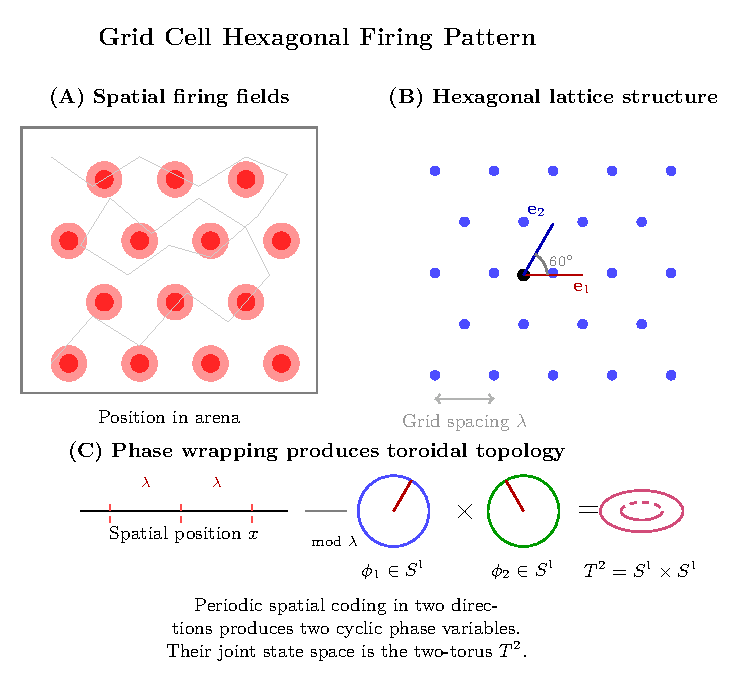
\includegraphics[width=\textwidth]{figures/fig_grid_cell_hex.pdf}
\caption{Grid cell hexagonal firing pattern. (A) Spatial firing fields of a single grid cell, showing elevated firing rates at regularly spaced locations forming a hexagonal lattice within the arena. (B) The hexagonal lattice structure defined by two basis vectors $\mathbf{e}_1$ and $\mathbf{e}_2$ separated by $60^\circ$, with characteristic grid spacing $\lambda$. (C) The periodic spatial code wraps each spatial direction modulo $\lambda$, producing two cyclic phase variables $\phi_1, \phi_2 \in S^1$. Their joint state space is the two-torus $T^2 = S^1 \times S^1$.}
\label{fig:grid_cell_hex}
\end{figure}

\subsection{The Gardner et al.\ Discovery: Methodology and Results}

Gardner et al.\ \cite{Gardner2022} used Neuropixels high-density silicon probes to record simultaneously from hundreds of grid cells in individual modules of the rat medial entorhinal cortex.
The key methodological innovation was the application of persistent cohomology to the high-dimensional population activity vectors.
Persistent cohomology is a tool from topological data analysis that identifies topological features (connected components, loops, voids) in a point cloud by tracking which features persist across a range of spatial scales.
For a dataset sampled from a torus, persistent cohomology detects two independent one-dimensional cocycles (corresponding to the two independent loops of the torus) that persist over a wide range of scales.

The analysis revealed that the joint activity of grid cells within a single module traces a path on a two-dimensional torus $T^2 = S^1 \times S^1$ (see Figure~\ref{fig:toroidal_manifold}).
The toroidal structure was robust across animals, recording sessions, and behavioral conditions, including periods of darkness when visual landmarks were unavailable.
This robustness confirmed that the toroidal geometry is an intrinsic property of the network dynamics rather than an artifact of external sensory input.

Subsequent work by Hermansen et al.\ \cite{Hermansen2024} extended the analysis to show that toroidal representations persist even during one-dimensional behavior, indicating that the toroidal structure is maintained by the network dynamics independently of the dimensionality of the behavioral task.
Di Sarra et al.\ \cite{DiSarra2025} demonstrated that oscillatory mechanisms play a role in maintaining the toroidal topology of grid cell population activity.

\begin{figure}[H]
\centering
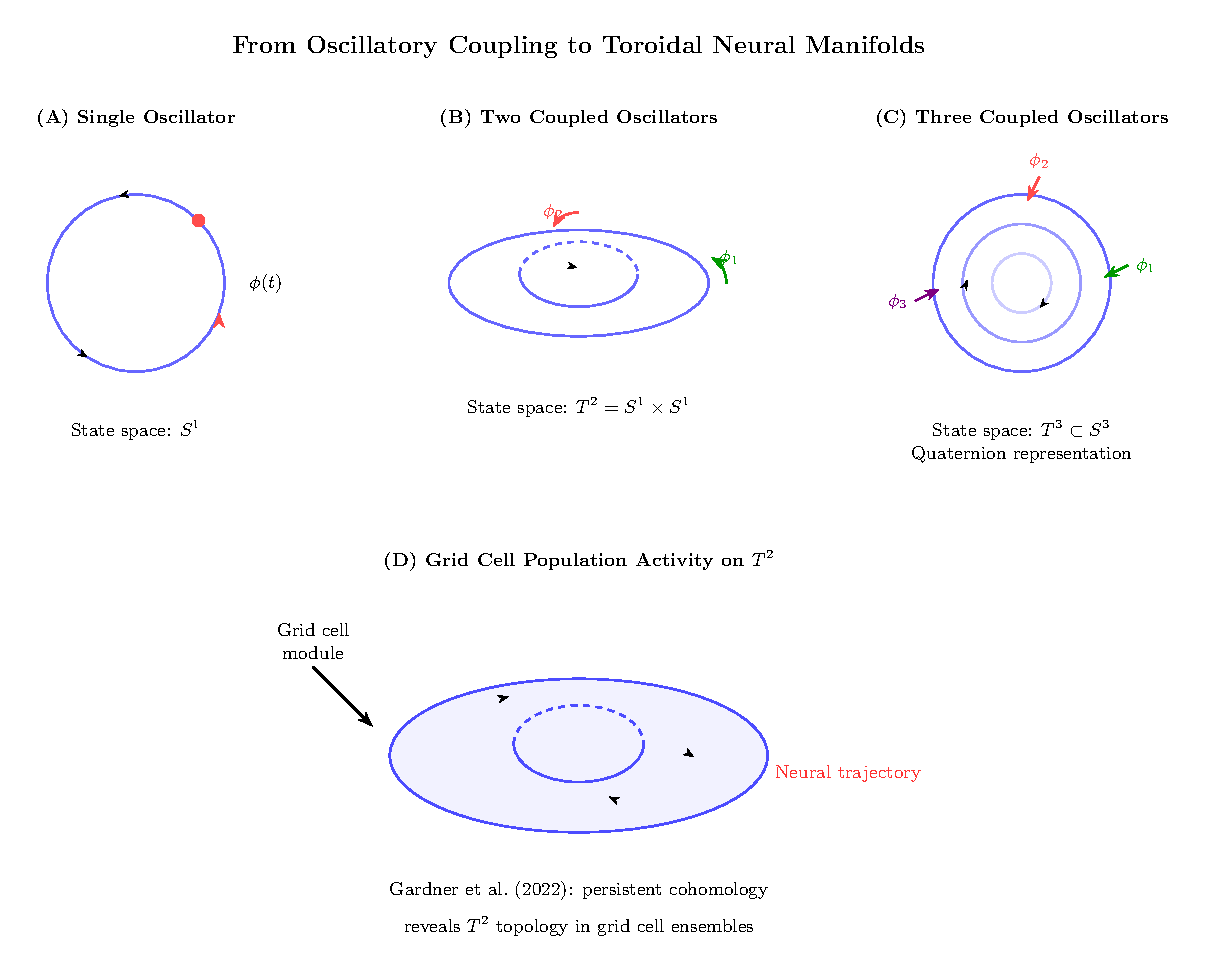
\includegraphics[width=\textwidth]{figures/fig_toroidal_manifold.pdf}
\caption{From oscillatory coupling to toroidal neural manifolds. (A) A single oscillator traces a circle $S^1$. (B) Two coupled oscillators produce dynamics on the two-torus $T^2 = S^1 \times S^1$. (C) Three coupled oscillators produce dynamics on $T^3 \subset S^3$, naturally represented by unit quaternions. (D) Grid cell population activity from a single module resides on a toroidal manifold, as demonstrated by Gardner et al.\ \cite{Gardner2022} using persistent cohomology.}
\label{fig:toroidal_manifold}
\end{figure}


%% ============================================================
%% SECTION 3: OSCILLATORY NEURAL DYNAMICS
%% ============================================================
\section{Oscillatory Neural Dynamics}\label{sec:oscillatory}

\subsection{The Electromagnetic Basis of Biological Dynamics}

At molecular and cellular scales, biological interactions are predominantly electromagnetic.
Chemical bonds arise from the overlap of electron wavefunctions governed by Coulomb forces; hydrogen bonds reflect dipole interactions; van der Waals forces result from fluctuating charge distributions \cite{Frohlich1968}.
The distinction between ``chemical'' and ``electromagnetic'' descriptions is one of abstraction level rather than ontological category.
By maintaining the electromagnetic framework as the base physical layer, it becomes possible to move continuously between molecular dynamics, neural activity, field interactions, and entropy flows without changing the fundamental descriptive language.

Living cells generate endogenous electromagnetic fields through several mechanisms.
Ion channel currents produce transient electric fields associated with action potentials, with typical neuronal membrane potentials of approximately $-70$~mV.
Charge transport in proteins, oscillatory metabolic activity, and membrane potential fluctuations all contribute to localized electromagnetic oscillations.
Whenever charges move, Maxwell's equations apply, and the resulting fields propagate according to the wave equation:
\begin{equation}\label{eq:wave}
  \nabla^2 \mathbf{E} - \mu_0 \epsilon_0 \frac{\partial^2 \mathbf{E}}{\partial t^2} = 0,
\end{equation}
where $\mathbf{E}$ is the electric field, $\mu_0$ is the permeability of free space, and $\epsilon_0$ is the permittivity of free space.
In biological tissue, the effective permittivity and conductivity are frequency-dependent, leading to complex dispersion relations that govern the propagation and attenuation of electromagnetic signals across different frequency regimes.

\subsection{The Frequency Hierarchy in Neural Systems}

The electromagnetic dynamics of neural tissue span an enormous range of frequencies.
Conventional electrophysiological methods access oscillatory activity primarily in the range of approximately 1 to $10^3$~Hz \cite{Buzsaki2006}.
These measurements have revealed a rich hierarchy of neural rhythms organized into canonical frequency bands, summarized in Table~\ref{tab:freq_bands}.

\begin{table}[H]
\centering
\caption{Canonical neural oscillation frequency bands accessible through conventional electrophysiology.}
\label{tab:freq_bands}
\begin{tabular}{lll}
\toprule
\textbf{Band} & \textbf{Frequency Range} & \textbf{Associated Functions} \\
\midrule
Delta ($\delta$) & 0.5--4 Hz & Deep sleep, cortical inhibition \\
Theta ($\theta$) & 4--8 Hz & Navigation, memory encoding \\
Alpha ($\alpha$) & 8--13 Hz & Relaxed wakefulness, sensory gating \\
Beta ($\beta$) & 13--30 Hz & Motor planning, active cognition \\
Gamma ($\gamma$) & 30--100 Hz & Sensory binding, attention \\
High gamma & 100--300 Hz & Local cortical computation \\
\bottomrule
\end{tabular}
\end{table}

Above the range of conventional electrophysiology, several intermediate frequency regimes remain poorly characterized in living neural tissue.
Ion channel kinetics and synaptic transmission dynamics operate in the kilohertz to megahertz range ($10^3$ to $10^6$~Hz).
Protein conformational vibrations, hydrogen bond network dynamics, membrane oscillations, and cytoskeletal lattice modes occur at still higher frequencies in the gigahertz to terahertz range ($10^{9}$ to $10^{13}$~Hz) \cite{Markelz2008, Frohlich1968}.

\subsection{Cross-Frequency Coupling}

The oscillatory bands listed in Table~\ref{tab:freq_bands} do not operate in isolation.
Cross-frequency coupling mechanisms link activity across bands, creating a hierarchical temporal organization.
The most extensively studied form is theta-gamma phase-amplitude coupling, in which the phase of theta oscillations modulates the amplitude of gamma bursts \cite{Canolty2006, Tort2009}.
This coupling allows slow oscillations to organize the timing of faster activity, creating nested temporal windows for information encoding \cite{Lisman2005}.

These coupled oscillatory dynamics are the physical substrate from which toroidal attractor manifolds emerge.
Each oscillatory band contributes a periodic phase variable, and the coupling between bands determines the trajectory on the resulting product manifold.
The mathematical formalization of this relationship is developed in the following sections.


%% ============================================================
%% SECTION 4: MATHEMATICAL TORUS CONSTRUCTION
%% ============================================================
\section{Mathematical Torus Construction}\label{sec:torus}

\subsection{From Circles to Tori: The Geometry of Periodic Coupling}

The connection between oscillatory dynamics and toroidal geometry follows from elementary topology.
Consider a single neural oscillator with phase variable $\theta_i(t)$ evolving as
\begin{equation}\label{eq:oscillator}
  \theta_i(t) = \omega_i t + \phi_i,
\end{equation}
where $\theta_i(t)$ is the instantaneous phase of the $i$-th oscillator, $\omega_i$ is its angular frequency, and $\phi_i$ is the initial phase offset.
Because $\theta_i$ is $2\pi$-periodic, it traces a trajectory on the circle $S^1$.
When two independent oscillators with phases $\theta_1(t)$ and $\theta_2(t)$ are considered jointly, each evolving on its own $S^1$, the state space of the combined system is the product manifold
\begin{equation}\label{eq:torus}
  T^2 = S^1 \times S^1,
\end{equation}
which is the two-dimensional torus. Two independent oscillators, each evolving on $S^1$, jointly span this product manifold because their combined state requires specifying two independent angles.
More generally, $n$ coupled periodic variables define a trajectory on the $n$-torus $T^n = (S^1)^n$ \cite{Strogatz2015}.

The torus $T^2$ can be embedded in three-dimensional Euclidean space via the standard parametric representation:
\begin{align}
  x(\theta, \phi) &= (R + r\cos\theta)\cos\phi, \label{eq:torus_x} \\
  y(\theta, \phi) &= (R + r\cos\theta)\sin\phi, \label{eq:torus_y} \\
  z(\theta, \phi) &= r\sin\theta, \label{eq:torus_z}
\end{align}
Here $R$ is the major radius, defined as the distance from the center of the torus to the center of the tube. The minor radius $r$ is the radius of the tube itself. The angles $\theta, \phi \in [0, 2\pi)$ correspond to the two independent phase variables.

\subsection{Coupled Oscillator Dynamics on the Torus}

This construction is not merely formal.
Whenever a physical system contains multiple oscillatory degrees of freedom, the natural state space for describing their joint dynamics is a torus.
The trajectory on this torus encodes the relative phase relationships between the oscillators.
If the frequency ratio between two oscillators is rational, the trajectory closes and the motion is periodic.
If the ratio is irrational, the trajectory never closes and instead densely fills the torus, producing quasi-periodic motion.
The distinction between these two cases has consequences for the information-carrying capacity of the system: quasi-periodic trajectories explore the full toroidal state space, while periodic trajectories are confined to lower-dimensional submanifolds.

For a system of two coupled oscillators with phases $\phi_1$ and $\phi_2$, the dynamics can be written in the general form:
\begin{align}
  \dot{\phi}_1 &= \omega_1 + \epsilon f_1(\phi_1, \phi_2), \label{eq:coupled1} \\
  \dot{\phi}_2 &= \omega_2 + \epsilon f_2(\phi_1, \phi_2), \label{eq:coupled2}
\end{align}
where $\omega_1$ and $\omega_2$ are the natural frequencies, $\epsilon$ is a coupling parameter, and $f_1, f_2$ are $2\pi$-periodic coupling functions.
The Kuramoto model \cite{Kuramoto1984, Strogatz2000} provides a canonical example in which $f_i$ depends on the phase difference $\phi_j - \phi_i$, leading to synchronization phenomena that have been extensively studied in the context of neural oscillations.


%% ============================================================
%% SECTION 5: KAM AND INVARIANT TORI
%% ============================================================
\section{KAM Theory and Invariant Tori}\label{sec:kam}

The persistence of toroidal motion under perturbation is guaranteed by the Kolmogorov--Arnold--Moser (KAM) theorem \cite{Kolmogorov1954, Arnold1963, Moser1962}.
For an integrable Hamiltonian system, each degree of freedom evolves quasi-periodically on an invariant torus according to
\begin{equation}\label{eq:quasiperiodic}
  \theta_i(t) = \omega_i t + \theta_{i,0}, \quad i = 1, \ldots, n,
\end{equation}
where $\theta_{i,0}$ are initial phases and $\bm{\omega} = (\omega_1, \ldots, \omega_n)$ is the frequency vector.
Trajectories remain confined to these invariant tori provided the frequencies are sufficiently incommensurate.
For sufficiently small perturbations and non-resonant frequency vectors, the majority of invariant tori persist. This is the content of the KAM theorem. The precise requirement is that the frequency vector satisfies a Diophantine condition:
\begin{equation}\label{eq:diophantine}
  |\bm{k} \cdot \bm{\omega}| \geq \frac{\gamma}{|\bm{k}|^\tau}, \quad \forall\, \bm{k} \in \mathbb{Z}^n \setminus \{\bm{0}\},
\end{equation}
where $\gamma > 0$ and $\tau > n - 1$.
This condition excludes frequency vectors with rational or near-rational ratios, which correspond to resonances where tori can be destroyed.

The relevance of the KAM framework to neural dynamics lies in the observation that neural oscillatory systems are weakly coupled: the coupling between distinct oscillatory populations is typically small relative to the intrinsic frequencies.
Under these conditions, the KAM theorem predicts that the toroidal structure of the combined phase space should persist, with quasi-periodic trajectories occupying most of the available state space.
The destroyed tori, corresponding to resonant frequency ratios, give rise to chaotic layers in phase space.
The coexistence of ordered toroidal regions and chaotic layers produces a mixed phase space structure that may be relevant to the balance between stable information encoding and flexible state transitions in neural systems.


%% ============================================================
%% SECTION 6: QUATERNION PHASE REPRESENTATION
%% ============================================================
\section{Quaternion Phase Representation}\label{sec:quaternions}

\subsection{Quaternions and Rotation Groups}

When three or more oscillatory bands are coupled simultaneously, the two-dimensional torus $T^2$ is insufficient to capture the full phase dynamics.
The state space of three coupled oscillators is the three-torus $T^3 = S^1 \times S^1 \times S^1$, which can be embedded in the three-sphere $S^3$.
Describing rotations and trajectories on $S^3$ requires a mathematical framework beyond ordinary complex numbers.
Quaternions provide such a tool.
A quaternion $q \in \mathbb{H}$ is a four-dimensional hypercomplex number of the form:
\begin{equation}\label{eq:quaternion}
  q = a + b\,\mathbf{i} + c\,\mathbf{j} + d\,\mathbf{k},
\end{equation}
where $a, b, c, d \in \mathbb{R}$ and the basis elements satisfy $\mathbf{i}^2 = \mathbf{j}^2 = \mathbf{k}^2 = \mathbf{i}\mathbf{j}\mathbf{k} = -1$.
Unit quaternions (those satisfying $|q| = 1$) form the three-sphere $S^3$, which is the universal cover of the rotation group $\mathrm{SO}(3)$.
Every rotation in three-dimensional space can be represented as conjugation by a unit quaternion:
\begin{equation}\label{eq:quat_rotation}
  \mathbf{v}' = q\,\mathbf{v}\,q^{-1},
\end{equation}
where $\mathbf{v}$ is a pure quaternion (with $a = 0$) representing a vector in $\mathbb{R}^3$.

\subsection{Quaternion Phase Representation of Coupled Oscillators}

Consider a system of three coupled oscillators with phases $\phi_1(t)$, $\phi_2(t)$, and $\phi_3(t)$.
The state of this system at any instant can be encoded as a unit quaternion:
\begin{equation}\label{eq:phase_quat}
  q(t) = \cos\!\left(\frac{\Phi}{2}\right) + \sin\!\left(\frac{\Phi}{2}\right)\left(n_1\,\mathbf{i} + n_2\,\mathbf{j} + n_3\,\mathbf{k}\right),
\end{equation}
where $(n_1, n_2, n_3)$ is a unit axis vector satisfying $n_1^2 + n_2^2 + n_3^2 = 1$, $\Phi$ is the composite rotation angle derived from the relative phases, and $q$ is unit normalized ($|q| = 1$).
The time evolution of $q(t)$ traces a trajectory on $S^3$.
When the oscillators are quasi-periodic, this trajectory lies on a torus embedded in $S^3$, generalizing the two-dimensional toroidal dynamics to higher dimensions.

The quaternion representation offers several advantages for describing coupled neural oscillatory dynamics.
Quaternion multiplication is non-commutative, reflecting the fact that the order in which phase rotations are composed matters for the resulting state.
This property is relevant to neural systems where the temporal sequence of phase relationships carries information \cite{Lisman2005}.
Quaternions avoid the gimbal lock singularities that arise in Euler angle representations, providing a smooth parameterization of the full rotation space.
The algebraic structure of quaternions naturally encodes the coupling between rotation axes, making it possible to represent interactions between oscillatory processes in different frequency bands as algebraic operations on quaternions.

\subsection{Quaternion Dynamics and the Three-Torus}

For a system of three quasi-periodic oscillators with incommensurate frequencies $(\omega_1, \omega_2, \omega_3)$, the trajectory in quaternion space traces a path on the three-torus $T^3 \subset S^3$.
The dynamics can be written as:
\begin{equation}\label{eq:quat_dynamics}
  \dot{q}(t) = \frac{1}{2}\,\bm{\Omega}(t)\,q(t),
\end{equation}
where $\bm{\Omega}(t) = \omega_1\,\mathbf{i} + \omega_2\,\mathbf{j} + \omega_3\,\mathbf{k}$ is a pure quaternion encoding the instantaneous angular velocity vector.
For uncoupled oscillators, $\bm{\Omega}$ is constant and the solution is a uniform flow on $T^3$.
Coupling between the oscillators introduces frequency-dependent corrections to $\bm{\Omega}$, producing the same type of quasi-periodic dynamics on perturbed tori that the KAM theorem describes in the Hamiltonian setting.

The extension to $n$ coupled oscillators requires the Clifford algebra $\mathrm{Cl}(n)$ or, equivalently, the consideration of trajectories on higher-dimensional tori $T^n$ embedded in higher-dimensional spheres.
The quaternion case ($n = 3$) is of particular interest for neural systems because it captures the minimal dimensionality needed to represent the simultaneous coupling of three frequency bands, such as the theta-gamma-alpha interactions observed in hippocampal and cortical circuits.

Table~\ref{tab:phase_dim} summarizes the relationship between the number of coupled oscillatory phases, the mathematical representation, and the resulting manifold geometry.

\begin{table}[H]
\centering
\caption{Relationship between coupled oscillatory phases, mathematical representation, and manifold geometry.}
\label{tab:phase_dim}
\begin{tabular}{cccc}
\toprule
\textbf{Phases} & \textbf{Representation} & \textbf{State Manifold} & \textbf{Neural Example} \\
\midrule
1 & Complex $e^{i\phi}$ & $S^1$ (circle) & Single rhythm \\
2 & $e^{i\phi_1} \times e^{i\phi_2}$ & $T^2$ (2-torus) & Grid cell module \\
3 & Unit quaternion $q$ & $T^3 \subset S^3$ & $\theta$-$\alpha$-$\gamma$ coupling \\
$n$ & Clifford algebra & $T^n$ & Multi-band interaction \\
\bottomrule
\end{tabular}
\end{table}


%% ============================================================
%% SECTION 7: THz MEASUREMENT GAP
%% ============================================================
\section{The Terahertz Measurement Gap}\label{sec:thz}

\subsection{The Frequency Hierarchy Beyond Conventional Electrophysiology}

Between the frequency range accessible through conventional electrophysiology and the molecular vibrational dynamics of neural tissue lies an observational gap spanning approximately 10 to 12 orders of magnitude (see Figure~\ref{fig:em_spectrum}).
EEG and related techniques measure activity up to roughly $10^3$~Hz, while molecular and lattice oscillations operate at $10^{9}$ to $10^{13}$~Hz.
The intervening range remains largely unexplored in living neural tissue, primarily because existing neuroscience instrumentation was not designed to detect signals at these frequencies.

Table~\ref{tab:freq_hierarchy} summarizes the full frequency hierarchy from conventional electrophysiology through molecular dynamics.

\begin{table}[H]
\centering
\caption{Electromagnetic frequency hierarchy in neural systems, from conventional electrophysiology to molecular dynamics.}
\label{tab:freq_hierarchy}
\begin{tabular}{lll}
\toprule
\textbf{Regime} & \textbf{Frequency Range} & \textbf{Physical Processes} \\
\midrule
EEG / LFP & $10^{0}$--$10^{3}$ Hz & Neural oscillations ($\delta, \theta, \alpha, \beta, \gamma$) \\
Ion channel dynamics & $10^{3}$--$10^{6}$ Hz & Channel gating, synaptic transmission \\
Measurement gap & $10^{6}$--$10^{9}$ Hz & Largely unexplored in living tissue \\
Molecular vibrations & $10^{9}$--$10^{13}$ Hz & Protein modes, H-bond networks, lattice modes \\
Optical / UV & $>10^{13}$ Hz & Electronic transitions \\
\bottomrule
\end{tabular}
\end{table}

\subsection{The Terahertz Band}

The terahertz band ($\sim 0.1$ to 10~THz) corresponds to photon energies of approximately 0.4 to 41~meV, a scale that matches thermal fluctuations in biological tissue, weak intermolecular forces, and hydrogen bond energies.
The characteristic wavelength at 1~THz is approximately 300~$\mu$m, which overlaps with cellular and tissue-scale organization.
Collective oscillatory modes in this frequency range can interact with mesoscopic biological structures without ionizing molecules, making them relevant to structural organization rather than chemical transformation.

Fr\"{o}hlich \cite{Frohlich1968} proposed that biological systems supplied with constant metabolic energy can produce coherent longitudinal electric modes in the frequency region between $10^{11}$ and $10^{12}$~s$^{-1}$.
Subsequent terahertz spectroscopy studies have confirmed that biological macromolecules exhibit collective vibrational modes in this frequency range \cite{Markelz2008}.
Sahu et al.\ \cite{Sahu2013} reported electromagnetic resonance measurements on single brain microtubules, identifying oscillatory behavior at frequencies consistent with lattice vibrational modes.
The existence of coherent Fr\"ohlich modes in living neural tissue remains an open experimental question.

The key observation is that current neuroscience instrumentation was not designed to detect signals in this intermediate range.
The terahertz band is of particular interest because it corresponds to collective vibrational modes of biological structures, and THz spectroscopy may reveal previously unobserved electromagnetic dynamics in neural tissue that are relevant to the synchronization landscape of macroscopic oscillatory activity.

\begin{figure}[H]
\centering
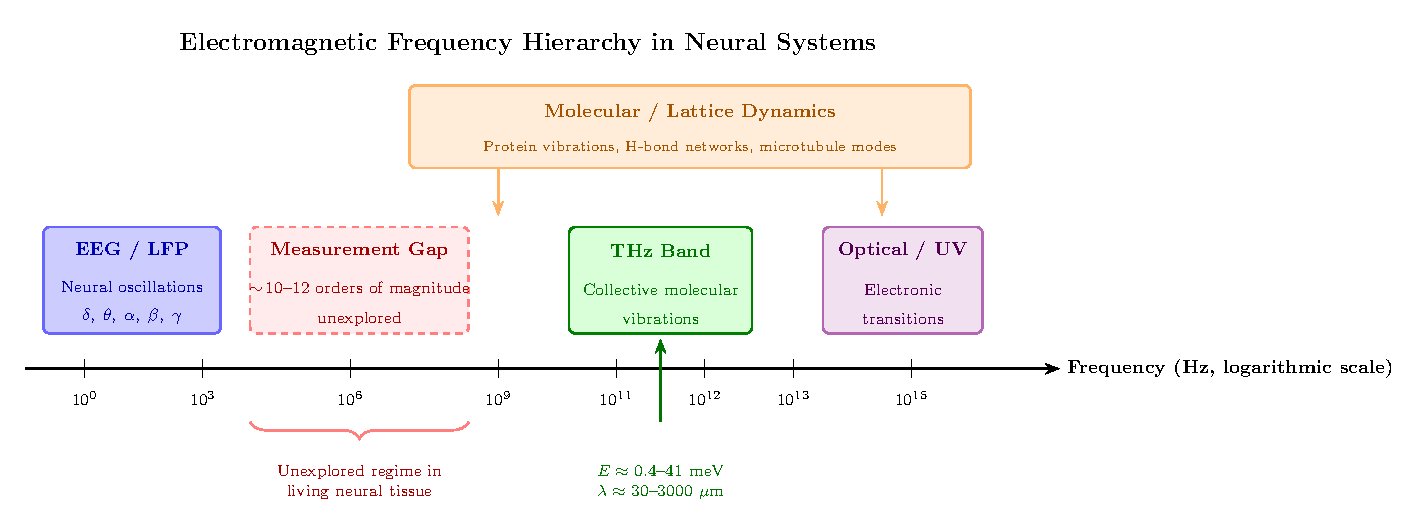
\includegraphics[width=\textwidth]{figures/fig_em_spectrum.pdf}
\caption{Electromagnetic frequency hierarchy in neural systems. The measurement gap between conventional electrophysiology (Hz to kHz) and molecular vibrational dynamics ($10^{9}$ to $10^{13}$~Hz) spans approximately 10 to 12 orders of magnitude. The terahertz band corresponds to collective molecular vibrations with photon energies matching thermal fluctuations and weak intermolecular forces in biological tissue.}
\label{fig:em_spectrum}
\end{figure}

\subsection{Multi-Scale Electromagnetic Coupling}

The framework presented here does not claim that terahertz radiation directly influences neural computation.
Rather, it proposes that the electromagnetic spectrum provides a continuous coordinate system for mapping biological dynamics across scales.
Low-frequency brain rhythms coordinate large-scale network states, while higher-frequency molecular dynamics encode finer structural information.
The electromagnetic spectrum bridges these layers, allowing the possibility that phase synchronization mechanisms operating at different frequency scales contribute to the overall organization of neural dynamics.

This multi-scale perspective aligns with established models of cross-frequency coupling in neural systems \cite{Canolty2006, Buzsaki2006}.
The extension is the recognition that the frequency hierarchy does not terminate at the upper boundary of conventional electrophysiology, but continues into regimes where collective molecular oscillations may influence the synchronization landscape of neural networks.
Energy flowing through the system produces oscillatory modes that, under far-from-equilibrium conditions, can form self-organized patterns consistent with the dissipative structures described by Prigogine \cite{Prigogine1977}.


%% ============================================================
%% SECTION 8: MICROBIOME EVOLUTIONARY PRESSURE
%% ============================================================
\section{Microbiome Evolutionary Pressure}\label{sec:gut_brain}

\subsection{The Microbial Ecosystem as an Internal Environment}

The human gastrointestinal tract harbors a microbial ecosystem of considerable complexity, comprising approximately $10^{13}$ to $10^{14}$ microorganisms representing thousands of species \cite{Cryan2019}.
This ecosystem fluctuates on timescales ranging from hours (in response to dietary intake) to years (in response to aging and environmental change).
The metabolic output of the gut microbiome includes short-chain fatty acids, neurotransmitter precursors (including serotonin, of which approximately 95\% is produced in the gut \cite{Yano2015}), immune signaling molecules, and a diverse array of metabolites that influence host physiology.

The vagus nerve provides a direct neural pathway between the gut and the brainstem, transmitting afferent signals from the enteric nervous system to the nucleus tractus solitarius and subsequently to higher brain regions \cite{Bonaz2018, Fulling2019}.
This gut-brain axis is bidirectional: descending vagal efferents modulate gut motility, secretion, and immune function, while ascending afferents convey information about the state of the gut ecosystem to the central nervous system \cite{Cryan2019, Mayer2011}.

\subsection{Evolutionary Pressure for Internal Recursive Modeling}

The argument advanced here goes beyond the established observation that the gut and brain are coupled \cite{Cryan2019, Bonaz2018, Dinan2017}.
The proposal is that the evolutionary pressure imposed by the need to manage a complex, fluctuating internal microbial ecosystem was a contributing driver of the neural pruning, hierarchical organization, and recursive internal modeling capacity that characterizes the mammalian brain.
The microbiome argument is presented as a plausible evolutionary pressure rather than a single causal driver.

An organism hosting a complex gut microbiome faces a continuous regulatory challenge.
The microbial ecosystem must be maintained within a functional range: too little microbial diversity compromises nutrient extraction and immune function; too much pathogenic activity threatens the host.
Managing this internal ecosystem requires the capacity to model the current state of the ecosystem, predict its trajectory, and generate appropriate regulatory responses.

The evolutionary pressure for this capacity is substantial.
Organisms with better internal models of their gut ecosystem would have been able to extract more nutrients, resist more pathogens, and maintain more stable metabolic states.
Over evolutionary time, this pressure would have favored nervous systems with greater capacity for hierarchical, recursive internal representation.

We propose that this evolutionary pressure contributed to the development of the modular, hierarchically organized oscillatory architecture observed in the mammalian brain.
The discrete frequency bands that characterize cortical oscillations \cite{Buzsaki2006} may reflect, in part, the need for a modular frequency regime capable of simultaneously representing information at multiple temporal scales.
The cross-frequency coupling mechanisms that link these bands \cite{Canolty2006, Tort2009} provide the recursive structure needed for hierarchical information integration \cite{Lisman2005}.

Table~\ref{tab:gut_brain} summarizes the proposed correspondence between gut ecosystem management demands and neural architectural features.

\begin{table}[H]
\centering
\caption{Proposed correspondence between gut ecosystem management demands and neural architectural features.}
\label{tab:gut_brain}
\begin{tabular}{ll}
\toprule
\textbf{Gut Ecosystem Demand} & \textbf{Neural Architectural Feature} \\
\midrule
Multi-scale temporal monitoring & Modular frequency bands ($\delta$ through $\gamma$) \\
Hierarchical state integration & Cross-frequency coupling \\
Predictive modeling of ecosystem & Recurrent attractor dynamics \\
Recursive internal representation & Hierarchical cortical organization \\
Continuous entropy management & Low-dimensional attractor manifolds \\
\bottomrule
\end{tabular}
\end{table}


%% ============================================================
%% SECTION 9: JAYNES AND RECURSIVE COGNITION
%% ============================================================
\section{Jaynes and Recursive Cognition}\label{sec:jaynes}

\subsection{The Jaynesian Framework}

Julian Jaynes \cite{Jaynes1976} proposed that human consciousness, in the modern introspective sense, is a relatively recent development in human history, emerging approximately 3,000 years ago during the late Bronze Age.
In Jaynes's account, earlier humans operated in a ``bicameral'' mode in which the right hemisphere generated auditory verbal hallucinations, experienced as the voices of gods or ancestors, that directed behavior. The left hemisphere executed these commands without the mediating layer of introspective self-awareness that characterizes modern consciousness.

The historical interpretation remains debated, but the computational distinction Jaynes identified is relevant.
What the Jaynesian framework usefully identifies is a computational transition: the emergence of a mode of neural processing in which the system can represent and reflect upon its own internal states.
The distinction between a neural architecture that cannot distinguish internally generated signals from external ones and an architecture that can is a genuine computational distinction with physical consequences.

\subsection{Modular Oscillatory Organization and the Consciousness Transition}

The framework developed in the preceding sections provides a physical mechanism for the transition Jaynes described.
In a nervous system without modular oscillatory organization, internal signals would be experienced as undifferentiated inputs, indistinguishable in kind from external sensory signals.
This corresponds to the bicameral state: internally generated verbal commands are experienced as external voices because the system lacks the architectural capacity to tag signals by their source.

The development of a modular frequency regime, with distinct frequency bands carrying information at different temporal scales and cross-frequency coupling providing hierarchical integration, creates the possibility of source attribution.
Signals arriving via different frequency channels can be distinguished by their spectral signature.
Internally generated signals, which originate from recurrent cortical processing and are embedded in the cross-frequency coupling structure, can be distinguished from externally driven signals, which enter the system through sensory pathways with different spectral characteristics.

This capacity for source attribution is the computational precondition for introspective consciousness.
When the system can distinguish internally generated representations from externally driven ones, it becomes possible to represent the fact that a given mental content is a product of the system's own processing.
This is the minimal form of self-reference: the system's representation of its own representational activity.

\subsection{Recursive Self-Reference and G\"odel-Type Structure}

G\"odel's incompleteness theorems \cite{Godel1931} demonstrate that any formal system of sufficient complexity to encode arithmetic can construct self-referential statements, and that such systems necessarily contain true statements that cannot be proven within the system.
This is a precise mathematical result about formal systems, not a general claim about physical systems.
Several authors, most notably Hofstadter \cite{Hofstadter1979} and Penrose \cite{Penrose1989}, have observed that the structural features underlying G\"odel's result have parallels in neural computation.

The neural framework developed here identifies a structural resemblance, not an equivalence, between self-referential formal systems and recursive neural dynamics.
A neural system with modular oscillatory organization and cross-frequency coupling can generate representations of its own oscillatory states, and these representations are themselves oscillatory states subject to the same dynamics.
This creates a recursive loop in which the system's model of itself is embedded within the system being modeled, a structure that resembles the self-referential encoding at the core of G\"odel's construction.

The toroidal attractor manifolds identified by Gardner et al.\ \cite{Gardner2022} provide a geometric substrate for this recursive structure.
A trajectory on a torus is inherently self-referential in the topological sense: it returns to previously visited regions of state space, and the pattern of returns encodes information about the global structure of the dynamics.
Quasi-periodic trajectories on tori never exactly repeat but continuously revisit neighborhoods of previous states, creating a form of approximate self-reference that is richer than simple periodicity.

We do not claim that neural systems are formal systems, or that G\"odel's theorems apply directly to neural computation.
Sufficiently complex recursive systems, whether formal or physical, share a structural feature: the capacity for self-reference generates both computational power and fundamental limitations.
In formal systems, self-reference produces true but unprovable statements.
In recursive neural systems, self-reference produces the capacity for introspective awareness but may also impose intrinsic limits on the completeness of self-knowledge.
This structural parallel is suggestive rather than deductive, and it indicates a direction for future investigation rather than a proven equivalence.

\begin{figure}[H]
\centering
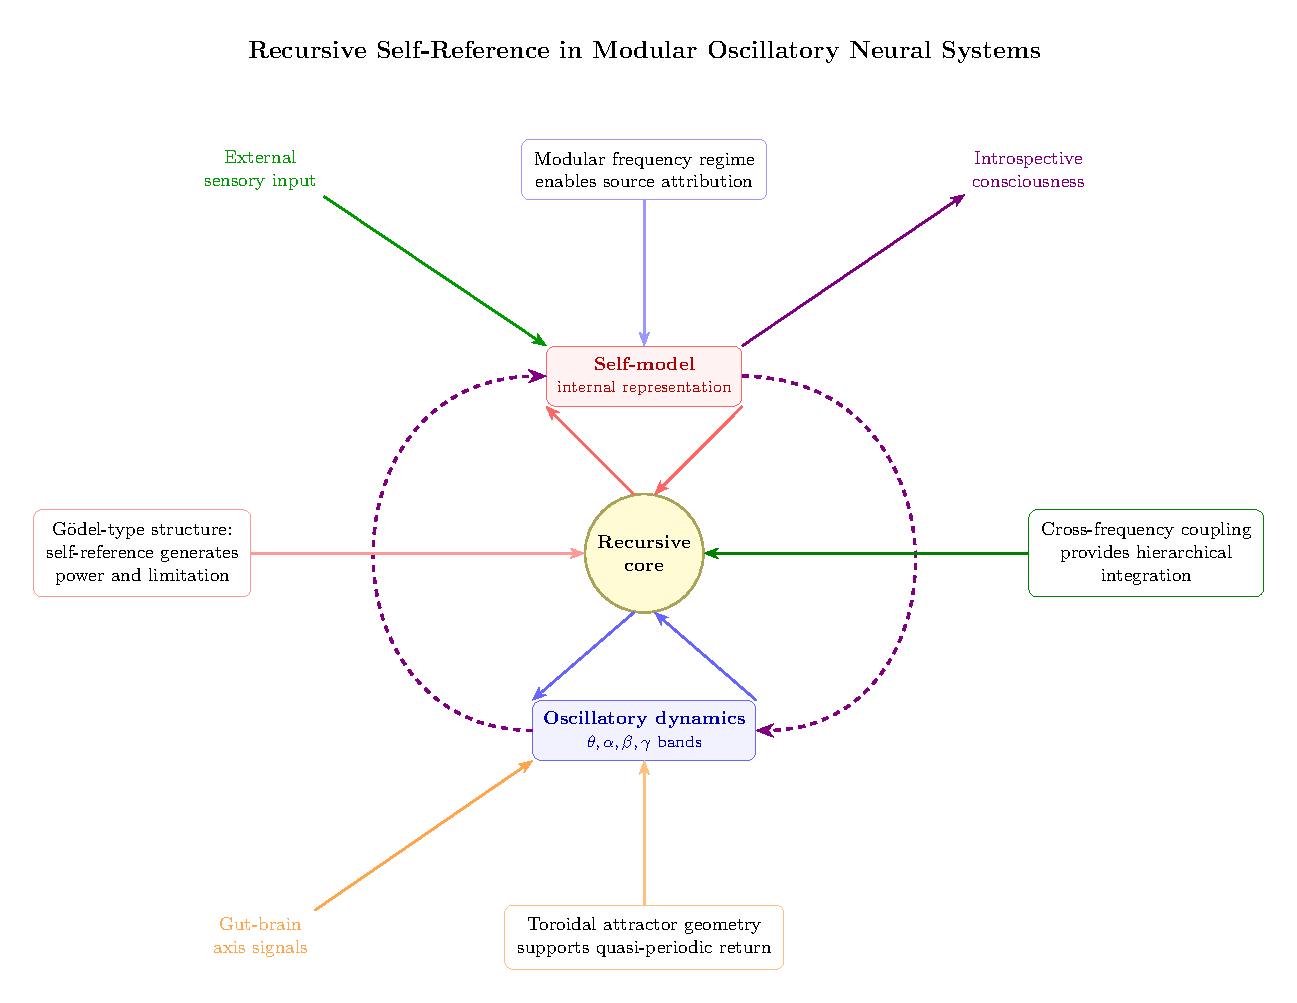
\includegraphics[width=0.85\textwidth]{figures/fig_recursive_loop.pdf}
\caption{Recursive self-reference in modular oscillatory neural systems. The system generates representations of its own oscillatory states (inner loop), which are themselves subject to the same oscillatory dynamics (outer loop). This recursive structure, enabled by modular frequency organization and cross-frequency coupling, provides the computational basis for introspective consciousness. The toroidal attractor geometry supports quasi-periodic trajectories that continuously revisit previous states without exact repetition, creating a physical analogue of G\"odel-type self-referential structure.}
\label{fig:recursive_loop}
\end{figure}


%% ============================================================
%% SECTION 10: ENTROPY AND ATTRACTOR STABILITY
%% ============================================================
\section{Entropy and Attractor Stability}\label{sec:entropy}

\subsection{Thermodynamic Constraints on Neural State Space}

Neural systems operate far from thermodynamic equilibrium, sustained by a continuous flow of metabolic energy.
The brain consumes approximately 20\% of the body's total metabolic output despite comprising roughly 2\% of body mass, reflecting the energetic cost of maintaining organized neural dynamics against the thermodynamic tendency toward entropy maximization.
This energetic investment is the physical precondition for the existence of structured attractor manifolds in neural state space.

From the perspective of nonequilibrium thermodynamics, the organized oscillatory patterns observed in neural systems are dissipative structures in the sense of Prigogine \cite{Prigogine1977}.
They maintain their organization by continuously dissipating energy, exporting entropy to the thermal environment while preserving internal order.
The entropy production rate $\dot{S}$ of a neural system can be decomposed into an internal entropy production term $\dot{S}_i \geq 0$ (required by the second law) and an entropy flux term $\dot{S}_e$ representing exchange with the environment:
\begin{equation}\label{eq:entropy_balance}
  \dot{S} = \dot{S}_i + \dot{S}_e.
\end{equation}
$S$ denotes thermodynamic entropy measured in units of Boltzmann's constant.
For a system maintaining a steady-state dissipative structure, $\dot{S} = 0$, which requires $\dot{S}_e = -\dot{S}_i < 0$: the system must export entropy at a rate equal to its internal entropy production.

\subsection{Entropy Gradients and Attractor Selection}

The existence of low-dimensional attractor manifolds in neural state space can be understood as a consequence of this entropy balance.
A high-dimensional neural system with $N$ neurons has a state space of dimension $N$.
However, the attractor manifolds on which the dynamics actually reside are typically of much lower dimension.
The toroidal manifold observed in grid cell populations \cite{Gardner2022} is two-dimensional, embedded in a state space whose dimension equals the number of simultaneously recorded neurons.
This dimensional reduction reflects the thermodynamic constraint: maintaining a high-dimensional attractor would require an entropy export rate that scales with the dimensionality, imposing an energetic cost that the system minimizes by confining its dynamics to low-dimensional manifolds.

The selection of specific attractor manifolds from the space of all possible low-dimensional structures is governed by the interplay between the system's dynamics and the entropy gradient landscape.
Northoff \cite{Northoff2019, Northoff2022} has proposed that the temporo-spatial dynamics of the brain's spontaneous activity define an entropy landscape in which different conscious states correspond to different entropy regimes.
The free-energy principle developed by Friston \cite{Friston2010} provides a complementary perspective, proposing that biological systems minimize variational free energy, a quantity that bounds the entropy of sensory states.

Among all possible low-dimensional attractor geometries, tori have special properties that make them thermodynamically favorable for information-processing systems.
Toroidal manifolds are compact (bounded and closed), ensuring that trajectories remain confined.
They support quasi-periodic motion, which provides a mechanism for encoding information in phase relationships without requiring the system to visit unstable fixed points.
They are structurally stable under perturbation (by the KAM theorem), meaning that the energetic cost of maintaining the attractor is minimized because the system does not need to actively correct for small perturbations.

\subsection{The Entropy Funnel}

The process by which high-dimensional neural activity is channeled onto low-dimensional attractor manifolds can be described as an entropy funnel (see Figure~\ref{fig:entropy_funnel}).
Raw neural activity, driven by sensory input, metabolic fluctuations, and intrinsic noise, initially occupies a high-dimensional region of state space.
Recurrent connectivity and oscillatory dynamics act as constraints that progressively reduce the effective dimensionality, channeling the activity onto attractor manifolds.
The entropy of the neural state decreases as the dimensionality is reduced, with the entropy difference being exported to the environment as heat.

This process is not passive.
The neural system actively maintains the attractor structure through synaptic plasticity, homeostatic regulation, and neuromodulatory control.
The metabolic cost of this maintenance represents the thermodynamic price of organized information processing.
Systems that achieve the same computational function on lower-dimensional attractors pay a lower metabolic cost, creating an evolutionary pressure toward efficient attractor geometries.

\begin{figure}[H]
\centering
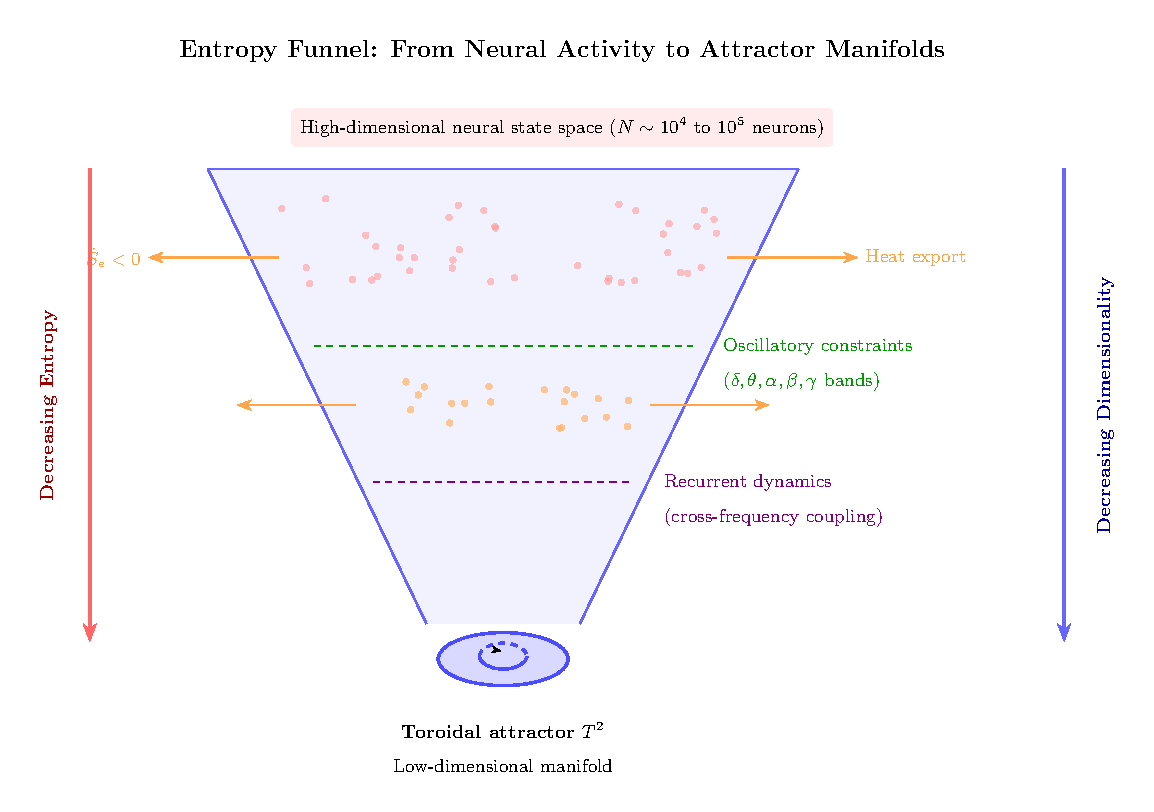
\includegraphics[width=0.85\textwidth]{figures/fig_entropy_funnel.pdf}
\caption{The entropy funnel: high-dimensional neural activity is progressively constrained by recurrent dynamics and oscillatory coupling onto low-dimensional attractor manifolds. The toroidal attractor $T^2$ represents a thermodynamically efficient geometry for encoding periodic information in phase relationships. Entropy decreases along the funnel axis as the effective dimensionality of the neural state is reduced.}
\label{fig:entropy_funnel}
\end{figure}


%% ============================================================
%% SECTION 11: TESTABLE PREDICTIONS
%% ============================================================
\section{Computational Pipeline and Ablation Studies}\label{sec:pipeline}

To validate the theoretical framework and demonstrate the extraction of toroidal manifolds from empirical data, we developed a complete, reproducible computational pipeline. The pipeline processes raw grid cell recordings, constructs firing rate maps, extracts the population manifold, computes topological features, and evaluates entropy metrics.

\subsection{Dataset and Preprocessing}
We analyzed the publicly available grid cell dataset from Hafting et al.\ (2005) \cite{Hafting2005}, which includes simultaneous recordings from the medial entorhinal cortex of freely foraging rats. The data consists of position timestamps, spatial coordinates, and spike times for individual neurons.

Preprocessing involved extracting position data and spike timestamps, aligning spikes to the nearest position sample, and removing all NaN values to ensure data integrity. The continuous position data was used to compute occupancy maps, while the aligned spike data provided the raw spike counts.

\subsection{Firing Rate Maps and Spatial Smoothing}
For each neuron, we constructed spatial firing rate maps by dividing the arena into a $50 \times 50$ grid. The raw spike count in each bin was divided by the occupancy time to compute the raw firing rate. To account for sampling noise and reveal the underlying spatial structure, we applied Gaussian smoothing ($\sigma = 2.0$) to the raw rate maps. This step is critical for visualizing the characteristic hexagonal firing fields of grid cells.

\subsection{Manifold Extraction and Persistent Homology}
To extract the population manifold, we constructed an activity matrix of shape (timepoints, neurons), where each entry represents the instantaneous firing rate of a neuron. We applied Principal Component Analysis (PCA) to reduce the dimensionality of the population activity, capturing the majority of the variance in the first three principal components.

We then applied persistent homology using the Ripser algorithm to the PCA-reduced manifold. Persistent homology computes the topological features of the data across multiple spatial scales, generating persistence barcodes and diagrams. The presence of long-lived features in the first homology group ($H_1$) indicates the existence of circular voids, which are the topological signatures of a toroidal manifold ($T^2 = S^1 \times S^1$).

\subsection{Entropy Metrics}
We computed three distinct entropy metrics to quantify the organization of the neural activity:
\begin{itemize}
    \item \textbf{Neural Entropy:} The Shannon entropy of the normalized population activity vector at each time step, measuring the instantaneous uncertainty of the population state.
    \item \textbf{Spatial Entropy:} The Shannon entropy of the normalized spatial firing rate map for each neuron, quantifying the uniformity of its spatial firing distribution.
    \item \textbf{Temporal Entropy:} The Shannon entropy of the binned spike train for each neuron, measuring the temporal irregularity of its firing.
\end{itemize}

\subsection{Ablation Studies}
To rigorously test the robustness of the manifold extraction and the necessity of the preprocessing steps, we conducted three ablation studies:

\textbf{1. No Smoothing:} We compared the raw, unsmoothed rate maps to the Gaussian-smoothed maps. Without smoothing, the hexagonal grid structure is heavily obscured by sampling noise, demonstrating that spatial smoothing is necessary to recover the underlying continuous attractor dynamics from discrete spike data.

\textbf{2. Reduced Neurons:} We evaluated the effect of population size on manifold reconstruction by performing PCA on subsets of neurons (e.g., 3, 5, 7, 10, 13). The cumulative variance explained by the top three principal components decreases as the number of neurons increases, reflecting the higher dimensionality of the raw state space. However, the underlying low-dimensional manifold structure remains stable, confirming that the toroidal topology is a robust property of the population, not an artifact of a specific subset of cells.

\textbf{3. Randomized Spikes:} We destroyed the temporal correlations in the data by randomly shuffling the spike times for each neuron independently. PCA on the shuffled data yielded a significantly different variance profile, and the resulting embedding lacked the structured geometry of the real manifold. Furthermore, the mean neural entropy of the shuffled data was lower than that of the real data, indicating that the structured, correlated firing of the real population occupies a specific, thermodynamically constrained region of state space that is lost upon randomization.

\section{Testable Predictions and Experimental Program}\label{sec:predictions}

A theoretical framework is only as valuable as the predictions it generates.
The synthesis presented in the preceding sections yields several concrete, experimentally testable predictions.

\textbf{Prediction 1: Toroidal manifolds beyond the entorhinal cortex.}
If the toroidal attractor framework reflects a general organizational principle, then persistent cohomology analysis applied to large-scale population recordings from other brain regions should reveal toroidal or higher-genus manifold structure.
Candidate regions include the prefrontal cortex during working memory maintenance, the motor cortex during rhythmic movement, and the hippocampus during temporal sequence encoding \cite{Bellmund2018}.

\textbf{Prediction 2: Phase coupling structure consistent with quaternion algebra in multi-band oscillatory data.}
If three or more oscillatory bands are simultaneously coupled in a manner consistent with quaternion dynamics, then the phase relationships should exhibit the non-commutative structure characteristic of quaternion multiplication.
This prediction can be tested using multi-electrode recordings with simultaneous theta, alpha, and gamma band decomposition \cite{Tort2009}.

\textbf{Prediction 3: Entropy gradient signatures during state transitions.}
The entropy funnel model predicts that transitions between conscious states should be accompanied by measurable changes in the effective dimensionality of neural population activity.
The transition from waking to deep sleep should correspond to a reduction in attractor dimensionality, while psychedelic states should correspond to an increase \cite{Northoff2022}.

\textbf{Prediction 4: Gut-brain axis perturbation affects attractor geometry.}
If the gut-brain axis contributes to the maintenance of oscillatory attractor structure, then perturbation of the gut microbiome should produce measurable changes in the geometry of neural attractor manifolds \cite{Cryan2019}.

\textbf{Prediction 5: THz-range collective modes correlate with oscillatory coherence.}
If collective molecular vibrations in the terahertz range contribute to the synchronization landscape of neural oscillations, then THz spectroscopy of neural tissue should reveal coherent modes whose properties correlate with the state of macroscopic oscillatory activity.

Table~\ref{tab:predictions} summarizes these predictions along with the experimental approaches needed to test them.

\begin{table}[H]
\centering
\caption{Testable predictions and corresponding experimental approaches.}
\label{tab:predictions}
\begin{tabular}{p{4cm}p{5cm}p{4cm}}
\toprule
\textbf{Prediction} & \textbf{Experimental Approach} & \textbf{Expected Outcome} \\
\midrule
Toroidal manifolds in non-entorhinal regions & Persistent cohomology on Neuropixels recordings & $T^2$ or higher-genus topology \\
Non-commutative phase coupling & Multi-band phase tensor analysis & Order-dependent coupling \\
Entropy gradient during state transitions & Dimensionality estimation (EEG/MEG) & Dim.~change with state \\
Gut perturbation affects attractors & Microbiome manipulation + neural recording & Attractor destabilization \\
THz modes correlate with coherence & THz spectroscopy of neural tissue & Coherent mode detection \\
\bottomrule
\end{tabular}
\end{table}


%% ============================================================
%% SECTION 12: CONCLUSION
%% ============================================================
\section{Conclusion: Toward a Physical Theory of Recursive Neural Organization}\label{sec:conclusion}

The framework developed in this paper connects five empirical and theoretical threads into a unified account of how self-referential information processing emerges from the physical dynamics of neural systems.

\textbf{Thread 1: Toroidal neural manifolds.}
The discovery by Gardner et al.\ \cite{Gardner2022} that grid cell population activity resides on a toroidal manifold $T^2$ established that non-trivial topological structure exists in neural population dynamics.
This finding is a concrete instance of a general principle: coupled oscillatory neural dynamics produce population activity organized on toroidal attractor manifolds, with the dimensionality of the torus reflecting the number of independent periodic variables encoded by the population.
Subsequent work by Hermansen et al.\ \cite{Hermansen2024} and Di Sarra et al.\ \cite{DiSarra2025} has confirmed that the toroidal structure is intrinsic to the network dynamics and is maintained by oscillatory mechanisms.

\textbf{Thread 2: Entropy-constrained attractor dynamics.}
The existence of low-dimensional attractor manifolds in high-dimensional neural state space reflects a thermodynamic imperative.
Neural systems, operating far from equilibrium as dissipative structures \cite{Prigogine1977}, must export entropy to maintain organized dynamics.
The energetic cost of maintaining an attractor scales with its dimensionality, creating evolutionary pressure toward low-dimensional manifolds.
Toroidal manifolds are thermodynamically favorable because they are compact, support quasi-periodic motion, and are structurally stable under perturbation (by the KAM theorem \cite{Kolmogorov1954, Arnold1963, Moser1962}).

\textbf{Thread 3: Modular oscillatory organization.}
The mammalian brain exhibits a hierarchical system of oscillatory frequency bands linked by cross-frequency coupling mechanisms \cite{Buzsaki2006, Canolty2006}.
This modular frequency regime provides the computational substrate for hierarchical information integration across temporal scales.
The mathematical representation of coupled multi-band dynamics naturally involves toroidal geometry (for two coupled phases), quaternion rotations (for three coupled phases), and higher-dimensional Clifford algebraic structures (for $n$ coupled phases).
The electromagnetic spectrum provides the physical substrate, with a significant measurement gap in the terahertz range that may conceal additional organizational mechanisms \cite{Frohlich1968, Markelz2008}.

\textbf{Thread 4: Evolutionary pressure from the gut-brain axis.}
The need to manage a complex, fluctuating internal microbial ecosystem imposed evolutionary pressure for neural architectures capable of hierarchical, recursive internal modeling \cite{Cryan2019}.
This pressure contributed to the development of the modular oscillatory organization observed in the mammalian brain.
The gut-brain axis argument is not about simple coupling between gut and brain; it is about the evolutionary demand for internal recursive modeling capacity driven by the complexity of the microbial ecosystem.

\textbf{Thread 5: The transition beyond primitive consciousness.}
The Jaynesian framework \cite{Jaynes1976} identifies a computational transition from a mode of neural processing in which internally generated signals are experienced as external commands to a mode in which they are recognized as products of the system's own activity.
The modular oscillatory organization described in Thread 3 provides the physical mechanism for this transition: distinct frequency channels enable source attribution, allowing the system to distinguish internally generated representations from externally driven ones.
This capacity for source attribution is the minimal form of recursive self-reference, enabled by the same toroidal attractor dynamics (Thread 1) operating under entropy constraints (Thread 2) that were shaped by evolutionary pressure from the gut-brain axis (Thread 4).

\textbf{The G\"odel connection.}
Introspective consciousness has a structural parallel in G\"odel's incompleteness theorems \cite{Godel1931}.
Sufficiently complex recursive systems, whether formal or physical, exhibit a common feature: self-reference generates both computational power and fundamental limitations.
The toroidal attractor geometry provides a physical substrate for this recursion. Quasi-periodic trajectories on tori continuously revisit previous states without exact repetition, creating a form of approximate self-reference bounded by the topology of the manifold.
As Hofstadter \cite{Hofstadter1979} argued, this recursive structure is a characteristic feature of systems capable of introspective representation.

These five threads converge on a single conclusion.
Grid cells empirically demonstrate that neural population dynamics can reside on toroidal manifolds.
Coupled oscillatory systems mathematically produce toroidal attractors.
Neural systems contain the oscillatory dynamics necessary for such manifolds to emerge.
Entropy constraints favor low-dimensional toroidal geometries as thermodynamically efficient substrates for information encoding.
The recursive self-reference enabled by modular oscillatory organization, shaped by evolutionary pressure for internal modeling, provides the computational architecture for introspective consciousness.

The framework is not complete.
The measurement gap in the terahertz range remains unexplored.
Toroidal manifold analysis has not yet been extended systematically beyond the entorhinal cortex.
The quaternion representation of multi-band coupling dynamics has not been tested experimentally.
The gut-brain evolutionary pressure argument requires further comparative analysis across species with varying microbiome complexity.
However, the framework generates concrete, testable predictions (Section~\ref{sec:predictions}) that can be addressed with current or near-future experimental technology.

Toroidal manifolds provide a physically grounded dynamical geometry for recursive neural computation.

\bibliographystyle{unsrtnat}
\bibliography{references}

\end{document}
